\documentclass{beamer}
\usepackage{graphicx}
\usepackage{xcolor}
\usepackage{tikz}

% 自定义颜色
\definecolor{purpleblue}{RGB}{80, 80, 180}
\definecolor{lightgray}{RGB}{230, 230, 230}
\definecolor{novelPurple}{RGB}{98, 54, 255} 
\definecolor{darkgray}{RGB}{50, 50, 50}

% 主题设置
\usetheme{Madrid}  
\usecolortheme{dolphin} 

% 设置字体（移除 fontspec，确保 pdfLaTeX 兼容）
\setbeamerfont{title}{size=\Large,series=\bfseries}
\setbeamerfont{frametitle}{size=\LARGE,series=\bfseries}
\setbeamercolor{frametitle}{fg=white, bg=novelPurple}
\setbeamercolor{title}{fg=white, bg=purpleblue}

% 封面信息
\title[SAT Hard Question]{\textbf{SAT Hard Question 9}}
\author{\textbf{Jack Zeng}}
\institute{\textcolor{white}{\textbf{Novel Prep}}}
\date{\today} 

\begin{document}

% --- Title Slide ---
\begin{frame}
    \titlepage
    \vfill
    \begin{flushright}
        \textcolor{purpleblue}{\Huge \textbf{Novel Prep}}
    \end{flushright}
\end{frame}


\begin{frame}
    \begin{tikzpicture}[remember picture, overlay]
        % 设置浅色渐变背景
        \shade[top color=softPurple, bottom color=softGray] 
            (current page.north west) rectangle (current page.south east);
        
        % 添加高斯模糊光晕
        \fill[white, opacity=0.3] (current page.center) circle (4cm);
        
        % 主标题
        \node[align=center] at (current page.center) {
            {\Huge\bfseries\textcolor{purpleblue}{Novel Prep}} \\[0.5cm]
            {\Large\itshape\textcolor{lightText}{Excellence in SAT Prep}}
        };

        % 添加柔和光点（点缀）
        \foreach \x in {1,2,3,4,5} {
            \fill[purpleblue, opacity=0.2] (rand*10-5, rand*7-3.5) circle (0.1+\x*0.05);
        }

        ;
    \end{tikzpicture}
\end{frame}


\begin{frame}{\textbf{Question : Exponential Growth}}
    \textbf{Elizabeth has \$4500 in an account.} \\
    Each year she expects to have **11\% more** money in the account than the previous year.  
    \vspace{0.3cm}
    \textbf{Which of the following models best describes how Elizabeth expects the money in her account to change over time?}
    
    \vspace{0.5cm}
    \begin{enumerate}
        \item[A.] Decreasing exponential
        \item[B.] Decreasing linear
        \item[C.] Increasing exponential
        \item[D.] Increasing linear
    \end{enumerate}
\end{frame}

\begin{frame}{\textbf{Answer Explanation}}
    \textbf{Correct Answer: \textcolor{novelPurple}{C. Increasing Exponential}}  

    \vspace{0.3cm}
    \textbf{Explanation:}
    \begin{itemize}
        \item \textcolor{red}{A. Decreasing exponential:} Incorrect, because the amount is increasing.
        \item \textcolor{red}{B. Decreasing linear:} Incorrect, because the amount is increasing, and the growth is not linear.
        \item \textcolor{green}{C. Increasing exponential:} **Correct!** The money grows by a fixed percentage each year.
        \item \textcolor{red}{D. Increasing linear:} Incorrect, because the growth is not constant but rather proportional.
    \end{itemize}
    
    \vspace{0.5cm}
    \textbf{Key Concept:} **Exponential growth occurs when a quantity increases by a fixed percentage each period.**
\end{frame}


\begin{frame}{\textbf{Question : Air Temperature and Altitude}}
    \textbf{The function} 
    \[
    T(x) = \frac{20,000 - 6.5x}{1,000}
    \]
    gives the estimated air temperature \( T(x) \), in degrees Celsius (°C), at an altitude of \( x \) meters.  

    \vspace{0.5cm}
    If the estimated temperature surrounding the hot air balloon is **15°C**, which of the following is closest to the altitude \( x \) of the hot air balloon?
    
    \vspace{0.5cm}
    \begin{enumerate}
        \item[A.] 20
        \item[B.] 769
        \item[C.] 1,333
        \item[D.] 5,385
    \end{enumerate}
\end{frame}

\begin{frame}{\textbf{Answer Explanation: Air Temperature}}
    \textbf{Correct Answer: \textcolor{novelPurple}{B. 769}}  

    \vspace{0.3cm}
    \textbf{Solution:}
    \[
    15 = \frac{20,000 - 6.5x}{1,000}
    \]
    Multiply both sides by 1,000:
    \[
    15,000 = 20,000 - 6.5x
    \]
    Solving for \( x \):
    \[
    x = \frac{20,000 - 15,000}{6.5} = \frac{5,000}{6.5} \approx 769.23
    \]
    Thus, the closest answer is **\( \mathbf{769} \)**.
\end{frame}


\begin{frame}{\textbf{Question : Finding a Possible Value of \( a + b \)}}
    The function \( f \) is defined as:
    \[
    f(x) = (x - a)(x - b)
    \]
    where \( a \) and \( b \) are integer constants.  

    \vspace{0.3cm}
    Given that:
    \[
    f(17) > 0, \quad f(20) < 0, \quad f(23) > 0
    \]
    What is one possible value of \( a + b \)?

    \vspace{0.5cm}
    \begin{enumerate}
        \item[A.] 39
        \item[B.] 38
        \item[C.] 37
        \item[D.] 36
    \end{enumerate}
\end{frame}

% --- Answer Explanation 2 ---
\begin{frame}{\textbf{Answer Explanation: Finding \( a + b \)}}
    \textbf{Correct Answer: \textcolor{novelPurple}{A. 39}}  

    \vspace{0.3cm}
    \textbf{Solution:}
    \[
    f(x) = (x - a)(x - b)
    \]
    The function changes sign at \( x = a \) and \( x = b \), meaning **\( f(x) \) is negative between \( a \) and \( b \)**.

    \vspace{0.3cm}
    Given:
    \[
    f(17) > 0, \quad f(20) < 0, \quad f(23) > 0
    \]
    This implies the roots are **between 17 and 23**, so we assume:
    \[
    a < 17, \quad b > 20
    \]
    Given \( a + b \) is an answer choice, we check:
    \[
    a + b = 39
    \]
    Which satisfies the conditions.  
\end{frame}

\begin{frame}{\textbf{Question: What Percent of \( b \) is \( a \)?}}
    The positive number \( a \) is 2,106\% of the sum of the positive numbers \( b \) and \( c \),  
    and \( b \) is 81\% of \( c \).  

    \vspace{0.3cm}
    What percent of \( b \) is \( a \)?

    \vspace{0.5cm}
    \textbf{Options:}
    \begin{enumerate}
        \item[A.] 4,706%
        \item[B.] 2,600%
        \item[C.] 38.12%
        \item[D.] 21.87%
    \end{enumerate}
\end{frame}

% --- Answer Explanation 11 ---
\begin{frame}{\textbf{Answer Explanation: What Percent of \( b \) is \( a \)?}}
    \textbf{Correct Answer:  \textcolor{novelPurple}{\( \mathbf{4,706\%} \)}}  

    \vspace{0.3cm}
    \textbf{Solution:}
    \begin{itemize}
        \item Given \( b = 0.81c \).
        \item Express \( a \) in terms of \( c \):
        \[
        a = 21.06(c + 0.81c) = 38.065c.
        \]
        \item Find \( \frac{a}{b} \):
        \[
        \frac{a}{b} = \frac{38.065c}{0.81c} = 47.06.
        \]
        \item Convert to percentage:
        \[
        a = 4706\%b.
        \]
    \end{itemize}
    \textbf{Final Answer:} \( \boxed{4,706\%} \).
\end{frame}

% --- Question 15 ---
\begin{frame}{\textbf{Question: Identifying the Base or Coefficient in \( f(x) \)}}
    For the function \( f \), for every increase of 2 in the value of \( x \),  
    the value of \( f(x) \) increases by a factor of \( c \), where \( c \) is a constant.  

    \vspace{0.3cm}
    Which of the following equivalent forms of function \( f \) displays the value of \( c \) as the base or the coefficient?

    \vspace{0.5cm}
    \textbf{Options:}
    \begin{enumerate}
        \item[A.] \( f(x) = 42(2)^{6x} \)
        \item[B.] \( f(x) = 42(8)^{2x} \)
        \item[C.] \( f(x) = 42(64)^x \)
        \item[D.] \( f(x) = 42(4096)^{\frac{x}{2}} \)
    \end{enumerate}
\end{frame}

% --- Answer Explanation 15 ---
\begin{frame}{\textbf{Answer Explanation: Identifying the Base or Coefficient in \( f(x) \)}}
    \textbf{Correct Answer: \textcolor{novelPurple}{\( \mathbf{f(x) = 42(4096)^{\frac{x}{2}}} \)}}  

    \vspace{0.3cm}
    \textbf{Solution:}
    \begin{itemize}
        \item Option A: \( 42(2)^{6x} \) - The base is \( 2^6 \), which is not what we need.
        \item Option B: \( 42(8)^{2x} \) - The base is \( 8^2 \), again incorrect.
        \item Option C: \( 42(64)^x \) - This is equivalent to \( 2^{6x} \), not the required form.
        \item Option D: \( 42(4069)^{\frac{x}{2}} \) - This correctly expresses the factor \( c \).
    \end{itemize}
    \textbf{Final Answer:} \( \boxed{42(4096)^{\frac{x}{2}}} \).
\end{frame}

\begin{frame}{\textbf{Question: Validity of a Research Study}}
    A study investigated the effect of magnesium supplementation on sleep quality.  
    190 adults were randomly selected, and their sleep efficiency was measured.  

    \vspace{0.3cm}
    Participants were randomly assigned to take a magnesium supplement or a placebo for 6 weeks.  
    The study concluded that magnesium improved sleep quality.  

    \vspace{0.5cm}
    What feature of this study supports this conclusion?

    \begin{itemize}
        \item[A.] There were more than 100 participants in the study.
        \item[B.] The participants were selected at random from the community center.
        \item[C.] The sleep efficiency of each participant was measured again at the end of 6 weeks.
        \item[D.] Each participant was randomly assigned to take a magnesium supplement or a placebo.
    \end{itemize}
\end{frame}

% --- Answer Explanation 16 ---
\begin{frame}{\textbf{Answer Explanation: Validity of a Research Study}}
    \textbf{Correct Answer: \textcolor{novelPurple}{\( \mathbf{D.} \)}}  

    \vspace{0.3cm}
    \textbf{Solution:}
    \begin{itemize}
        \item **Random assignment** ensures that the two groups (magnesium vs. placebo)  
        were similar at the start, meaning that any difference in sleep quality at the end  
        can be attributed to the magnesium supplement.
        \item This eliminates confounding variables and makes it possible to conclude  
        that magnesium caused the improvement.
    \end{itemize}
    \textbf{Final Answer:} \( \boxed{D} \).
\end{frame}



% --- Question 17 ---
\begin{frame}{\textbf{Question: Finding a Point on Line \( t \)}}
    A circle in the \( xy \)-plane has its center at \( (-1,1) \).  
    Line \( t \) is tangent to this circle at the point \( (7,-6) \).  

    \vspace{0.3cm}
    Which of the following points also lies on line \( t \)?

    \vspace{0.5cm}
    \begin{itemize}
        \item[A.] \( (0,7) \)
        \item[B.] \( (6,9) \)
        \item[C.] \( (14,2) \)
        \item[D.] \( (15,1) \)
    \end{itemize}
\end{frame}

% --- Answer Explanation 17 ---
\begin{frame}{\textbf{Answer Explanation: Finding a Point on Line \( t \)}}
    \textbf{Correct Answer: \textcolor{novelPurple}{\( \mathbf{C. (14,2)} \)}}  

    \vspace{0.3cm}
    \textbf{Solution:}
    \begin{itemize}
        \item Compute the slope from the center \( (-1,1) \) to the tangent point \( (7,-6) \):
        \[
        \frac{-6 - 1}{7 - (-1)} = \frac{-7}{8}.
        \]
        \item The slope of line \( t \) is the negative reciprocal:
        \[
        \frac{8}{7}.
        \]
        \item Equation of line \( t \) using \( (7,-6) \):
        \[
        y + 6 = \frac{8}{7}(x - 7).
        \]
        \item Solve for \( (14,2) \)
    \end{itemize}
 
\end{frame}

% --- Question 18 ---
\begin{frame}{\textbf{Question: Solving for \( a + b + c \)}}
    The function \( f(x) \) is defined by:
    \[
    f(x) = \frac{x^2 + ax + b}{2x + c},
    \]
    where \( a, b, \) and \( c \) are constants.  

    \vspace{0.3cm}
    The graph of \( f(x) \) does not intersect the line \( x = 4 \).  
    If \( f(5) = f(6) = 0 \), what is the value of \( a + b + c \)?

    \vspace{0.5cm}
    \begin{itemize}
        \item[A.] 10
        \item[B.] 11
        \item[C.] 12
        \item[D.] 13
    \end{itemize}
\end{frame}

% --- Answer Explanation 18 ---
\begin{frame}{\textbf{Answer Explanation: Solving for \( a + b + c \)}}
    \textbf{Correct Answer: \textcolor{novelPurple}{\( \mathbf{B. 11} \)}}  

    \vspace{0.3cm}
    \textbf{Solution:}
    \begin{itemize}
        \item Since \( f(x) \) does not intersect \( x = 4 \), the denominator must be 0 at \( x = 4 \):
        \[
        2(4) + c = 0 \implies c = -8.
        \]
        \item Given \( f(5) = 0 \) and \( f(6) = 0 \), set the numerator to 0:
        \[
        5^2 + 5a + b = 0, \quad 6^2 + 6a + b = 0.
        \]
        \item Solve:
        \[
        25 + 5a + b = 0,
        \]
        \[
        36 + 6a + b = 0.
        \]
        \item Subtract equations:
        \[
        (36 + 6a + b) - (25 + 5a + b) = 0.
        \]
        \[
        11 + a = 0 \implies a = -11.
        \]

    \end{itemize}

\end{frame}

\begin{frame}{Answer Explanation: Solving for \( a + b + c \)} 
\begin{itemize}
        \item Find \( b \):
        \[
        25 + 5(-11) + b = 0 \implies b = 30.
        \]
        \item Compute sum:
        \[
        a + b + c = -11 + 30 + (-8) = 11.
        \]
    \end{itemize}
    
\end{frame}


\begin{frame}{\textbf{Question: Finding \( r + t \)}}
    The shaded region represents the solutions to the inequality:
    \[
    r x + t y \geq -65
    \]


    

    \vspace{0.3cm}
    What is the value of \( r + t \)?

    \begin{center}
        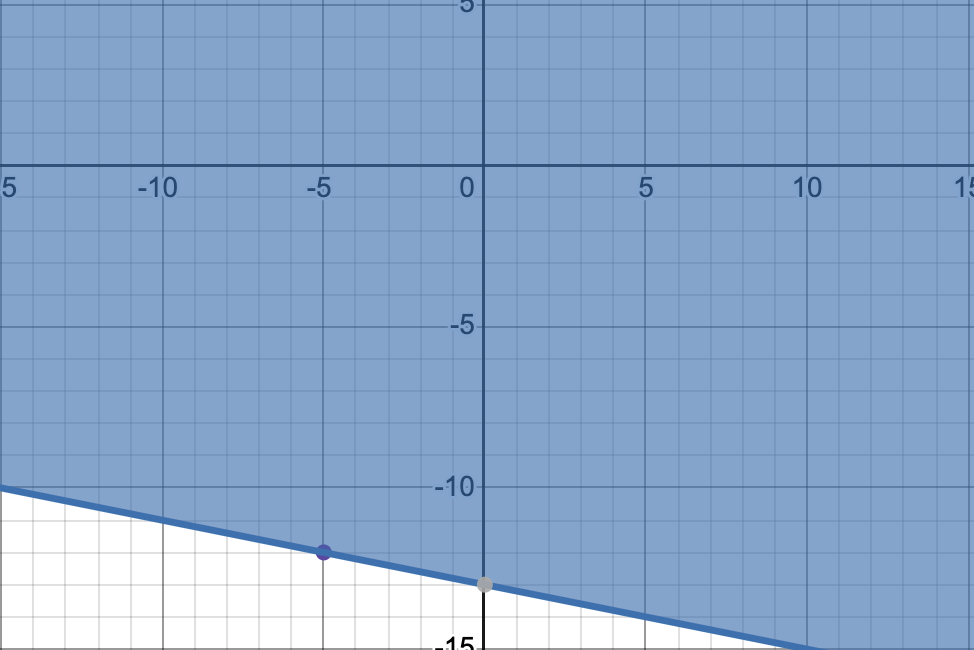
\includegraphics[width=0.4\linewidth]{f7.png}
    \end{center}

    

    \vspace{0.5cm}
    \begin{itemize}
        \item[A.] 6
        \item[B.] 4
        \item[C.] -4
        \item[D.] -5
    \end{itemize}
\end{frame}

% --- Answer Explanation 12 ---
\begin{frame}{\textbf{Answer Explanation: Finding \( r + t \)}}
    \textbf{Correct Answer: \textcolor{novelPurple}{\( \mathbf{A. 6} \)}}  

    \vspace{0.3cm}
    \textbf{Solution:}
    \begin{itemize}
        \item The boundary line of the shaded region is given by:
        \[
        r x + t y = -65.
        \]
        \item The line passes through the points \( (-5,-12) \) and \( (0,-13) \).
        \item Substituting these into the equation:
        \[
        r(-5) + t(-12) = -65, \quad r(0) + t(-13) = -65.
        \]
        \item Solving for \( r \) and \( t \):
        \[
        t = 5, \quad r = 1.
        \]
        \item Compute the sum:
        \[
        r + t = 6.
        \]
    \end{itemize}
    \textbf{Final Answer:} \( \boxed{6} \).
\end{frame}




\end{document}

